\cotefile{36}
\scanpage{3}
\mspage{1}
\margin{\figure{\begin{tikzpicture}\draw (0,0) .. controls (.1,-.2) and (.4,-.35) .. (.6,-.65);\end{tikzpicture}}}

\uline{Remarques.\qquad SGA 7 $\overline{\underline{\mathrm{IX}}}$}

0.

i).\quad Dire que $\ell$ est un nombre premier à $p$ (pour que
$\begin{array}[t]{r}\ell\,6\\ \ell\,7\\ \text{ii)}\ \ell\,3\end{array}$
soit OK p.e.)

Pourquoi $S$ \unsure{hensélien|Limélien} ?

$0.1,\ \ell\,9$ : pourquoi seulement à isogénie près ? (si $\ell\ne p$ ; \deleted{)} sinon ce ne veut rien dire)

. $\ell\,14$ : il semble clair\qquad est un peu optimiste.

ii).\quad $\ell\,14$\quad français :\qquad et qui\qquad ($\,;\,$ il\quad ?)

iii).\quad \begingroup
\setbox0=\hbox{$\ell\,6$}
\hbox{\rlap{
\begin{tikzpicture}[overlay,baseline=0pt]
\draw[gray,line width=.35pt] (\dimexpr\wd0+9pt\relax,12pt) .. controls (\dimexpr\wd0+4pt\relax,25pt) and (-15pt,15pt) .. (-13pt,-9pt);
\draw[line width=.65pt] (-13pt,-9pt) .. controls (-14pt,-16pt) and (-3pt,-16pt) .. (\dimexpr\wd0-3pt\relax,-12pt);
\draw[gray,line width=.35pt] (\dimexpr\wd0-3pt\relax,-12pt) .. controls (\dimexpr\wd0+12pt\relax,-7pt) and (\dimexpr\wd0+15pt\relax,5pt) .. (\dimexpr\wd0+13pt\relax,13pt);
\end{tikzpicture}}\box0}
\endgroup\quad
une référence ou définition pour réduction semi-stable d'une courbe (seule la terminologie de ``réduction stable'' se trouve dans [3])

iv)\quad $\ell\,12$\quad orthographe ?\qquad système

\begingroup
\setbox0=\hbox{$\ell\,15$}
\hbox{\rlap{\begin{tikzpicture}[overlay,baseline=0pt]
\draw[line width=.5pt] (-13pt,-5pt) .. controls (-21pt,2pt) and (-2pt,11pt) .. (8pt,14pt) .. controls (\dimexpr\wd0+14pt\relax,27pt) and (\dimexpr\wd0+20pt\relax,-5pt) .. (\dimexpr\wd0+5pt\relax,-13pt);
\draw[gray,line width=.35pt] (\dimexpr\wd0+5pt\relax,-13pt) .. controls (5pt,-20pt) and (-10pt,-13pt) .. (-12pt,-9pt);
\end{tikzpicture}}\box0}
\endgroup\quad vider la Rmq sur les $H^i$ (qui n'est ni
\begin{tikzpicture}[baseline=0pt,overlay,x=1em,y=1ex]
\draw[gray] (8.3,2.8) .. controls (5.7,5.4) and (-.8,3.7) .. (-.5,.7)
.. controls (-.7,-1.5) and (6.5,-1.5) .. (8.0,1.8)
.. controls (8.4,2.5) and (7.7,3.1) .. (6.8,3.3);
\end{tikzpicture}liée à la \inserted{?}monodromie, ni fondé sur des théorèmes)

\figure{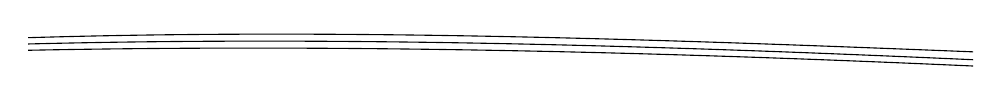
\begin{tikzpicture}
\draw (0,0) .. controls (4,.12) and (8,-.02) .. (12,-.18);
\draw (0,-.08) .. controls (4,.02) and (8,-.10) .. (12,-.28);
\draw (0,-.16) .. controls (4,-.08) and (8,-.18) .. (12,-.36);
\end{tikzpicture}}

1.

\uline{p 0}.\quad titre :\qquad $\ell'$ (minuscule)

$(1.0)\ \ell\,5$\qquad donc\qquad ?

\begingroup
\setbox0=\hbox{$\ell\,7$}
\hbox{\rlap{\begin{tikzpicture}[overlay,baseline=0pt]
\draw[gray,line width=.4pt] (\dimexpr\wd0+8pt\relax,16pt) .. controls (\dimexpr\wd0+2pt\relax,27pt) and (-21pt,10pt) .. (-14pt,-10pt) .. controls (-4pt,-24pt) and (\dimexpr\wd0+18pt\relax,-1pt) .. (\dimexpr\wd0+10pt\relax,13pt);
\draw[line width=.3pt] (-15pt,-13pt) -- (\linewidth,-13pt);
\end{tikzpicture}}\box0}
\endgroup\quad à quel concept se rapporte ``lequel''.

\smallskip

\uline{p1}\quad $\ell\,12$\quad français : choisie\quad ; ``qui est'' tend à faire croire qu'on impose une condition supplémentaire

$\ell\,16$\quad $=B$ donc le symbole est malheureux;\quad $=A'_K$ de toute façon.

\rule{\linewidth}{0.3pt}

p2.\quad $\ell\,2$\quad pourquoi \begingroup
\setbox0=\hbox{G}
\hbox{\rlap{\begin{tikzpicture}[overlay,baseline=0pt]
\draw[gray,line width=.35pt] (0pt,13pt) .. controls (-8pt,9pt) and (-5pt,-6pt) .. (3pt,-6pt) .. controls (\dimexpr\wd0+8pt\relax,-3pt) and (\dimexpr\wd0+8pt\relax,14pt) .. (\dimexpr\wd0-1pt\relax,14pt) .. controls (3pt,14pt) and (3pt,12pt) .. (2pt,11pt);
\end{tikzpicture}}\box0}
\endgroup{}roupe
\quad -- épimorphisme n'est pas la définition d'isogénie --

$\ell\,15$\quad -- supprimer séparé type fini au bénéfice du seul quasi projectif.

-- que $A\mathbin{\underset{S}{\times}}\operatorname{Spec}(K)\xrightarrow{\sim}A_K$ est une trivialité

\margin{2}
